\documentclass[
	parskip=half,
	a4paper,
]{scrarticle}

\usepackage{xcolor}
\definecolor{seeblau}{HTML}{00A9E0}
\definecolor{seegrau}{HTML}{9AA0A7}

\definecolor{seeblau1}{HTML}{CCEEF9}
\definecolor{seeblau2}{HTML}{A6E1F4}
\definecolor{seeblau3}{HTML}{59C7EB}
\definecolor{seeblau4}{HTML}{00A9E0}
\definecolor{seeblau5}{HTML}{008ECE}


\usepackage{graphicx}
\usepackage{amsmath}
\usepackage{subcaption}
\usepackage{wrapfig}
\usepackage[english]{babel}
\usepackage{blindtext}
\usepackage{microtype}
\usepackage{siunitx}
\usepackage[utf8]{inputenc}
\usepackage{csquotes}
\usepackage{nicefrac}
\usepackage[T1]{fontenc}
\usepackage{amsfonts}
\usepackage{amssymb}
\usepackage{tikz}
\usepackage{parskip}

\usepackage{libertinus, libertinust1math}
\usepackage[sfdefault]{biolinum}
\usepackage{roboto}

\setkomafont{disposition}{\normalfont\sffamily}

% set margins
\usepackage{geometry}
\geometry{
	a4paper,
	left=2.5cm,
	right=2.5cm,
	top=2.5cm,
	bottom=2.5cm
}

% caption
\usepackage{caption}
\captionsetup{
	% font={sf},
	labelfont={sf, bf, color=seeblau},
	labelsep=quad,
	labelformat=simple,
}

% links
\usepackage{hyperref}
\hypersetup{
	colorlinks=true,
	linkcolor=seeblau,
	citecolor=seeblau,
	urlcolor=seeblau,
	% hidelinks=true
}

% bibliography
\usepackage[
	style=numeric-comp, % comp = compressed 4,5,6,7 -> 4-7
	sorting=none,		% Sort by appearance
	% autocite = superscript,
	% backref=true,
	hyperref=true,
	url=true,
	maxbibnames=100
]{biblatex}

\usepackage{float}
% \floatplacement{figure}{h}
% \floatplacement{table}{H}

% loosen float placement rules
\renewcommand{\topfraction}{0.8}
\renewcommand{\bottomfraction}{.8}
\renewcommand{\textfraction}{0.1}
\renewcommand{\floatpagefraction}{.9}
% make floats less likely to be placed on a separate page
\setcounter{totalnumber}{9}
\setcounter{topnumber}{9}
\setcounter{bottomnumber}{9}

% decrease space between floats and text
\setlength{\textfloatsep}{0.25cm}
\setlength{\floatsep}{0.25cm}

% decrease space after disposition
\RedeclareSectionCommands[
	afterskip=1px
]{section, subsection, subsubsection}

\usepackage{adjustbox}

\usepackage{datetime}
\newdateformat{dotdate}{
	\twodigit{\THEDAY}.\twodigit{\THEMONTH}.\THEYEAR
}
\newdateformat{monthyeardate}{%
  \monthname[\THEMONTH] \THEYEAR}


% header and footer
\usepackage[
  markcase=noupper
]{scrlayer-scrpage}% activates pagestyle scrheadings automatically
\clearpairofpagestyles
\setkomafont{pageheadfoot}{\normalfont\sffamily}
\setkomafont{pagenumber}{\normalfont\sffamily}
% \chead*{\color{seegrau} Draft \dotdate\today}
\ofoot*{\pagemark}
\ohead*{\rightmark}


\usepackage{ifthen}
\newcommand{\markieren}[4]{
	\ifthenelse{\equal{#1}{}}{}{\adjustbox{padding=3pt, bgcolor=seeblau1, margin=-1pt}{\strut{\sffamily\robotoMedium{#1}}}\\}
  \ifthenelse{\equal{#2}{}}{}{\adjustbox{padding=3pt, bgcolor=seeblau2, margin=-1pt}{\strut{\sffamily\robotoMedium{#2}}}\\}
	\ifthenelse{\equal{#3}{}}{}{\adjustbox{padding=3pt, bgcolor=seeblau3, margin=-1pt}{\strut{\sffamily\robotoMedium{#3}}}\\}
	\ifthenelse{\equal{#4}{}}{}{\adjustbox{padding=3pt, bgcolor=seeblau4, margin=-1pt}{\strut{\sffamily\robotoMedium{#4}}}}
}

\addbibresource{../literature.bib}
\begin{document}

\title{Ultrafast Photoluminescence}
\author{Leon Oleschko}
\date{\dotdate\today}

\begin{titlepage}
    \sffamily
    \vspace*{3cm}
    {
        \fontsize{32}{32}
        \markieren{}{}{Ultrafast}{Photoluminescence}
    }
    \vspace{.25cm}\\
    {
        \Large
        Leon Oleschko\\
        supervised by Peter Baum
        \vspace{.05cm}\\
        \dotdate\today\\
        \textbf{Draft}\\
        \vspace{.05cm}\\
        \normalsize
        Projekt Praktikum\\
        Universität Konstanz
    }
    \vfill
    {
        \normalfont\normalsize
    }
    \vfill
    \begin{flushright}
        Available at \url{www.github.com/leoole100/projekt-praktikum}.
    \end{flushright}
\end{titlepage}

% {
% 	\sffamily
% 	\hypersetup{hidelinks}
% 	\tableofcontents
% }

\clearpage

\section{Introduction}


\clearpage
\section{Model}
% To obtain the spectral shape, the ultrafast absorption and subsequent thermal emission is modelled with a zero-dimensional (lumped) two-temperature picture for the probed volume. The probed volume is approximated as the excited spot area times the optical absorption depth, \(V_{\text{probe}} \approx A_{\text{spot}}\,d_{\text{abs}}\). A short laser pulse deposits power \(P(t)\) into the electronic system, which rapidly thermalizes; electron–phonon coupling then cools the electrons toward the lattice temperature \(T_l\)~\cite{kampfrathStronglyCoupledOptical2005}. Neglecting transport and other slow losses on the picosecond timescale, the electron temperature \(T_e(t)\) obeys
\begin{equation}
    \frac{\mathrm d T_e(t)}{\mathrm d t}
    \;=\;
    -\,\frac{T_e - T_l}{g}
    \;+\;
    \frac{P(t)}{C_e(T_e)}.
    \label{eq:Te}
\end{equation}
% Here \(C_e(T_e)\) is the electronic heat capacity of the probed volume (units \si{J\per K}), \(g\) is the electron–phonon energy-relaxation time, \(T_l\) is the lattice temperature (taken approximately constant over this window since typically \(C_l \gg C_e\)), and \(P(t)\) is the laser power deposited in the probed volume (units \si{W}).\\
% Because the instantaneous radiant exitance scales with \(T^4\) (Stefan–Boltzmann law), the emission is dominated by the high-temperature portion of \(T_e(t)\) immediately after excitation; the later, lower-temperature evolution contributes comparatively little. This justifies treating \(T_l\) as constant and using the simplified dynamics above when we are interested in the relative spectral shape rather than absolute irradiance. \cite{roobThermalRadiationUltrafast2025}

% To map \(T_e(t)\) to the emitted spectrum we use Planck’s law. The blackbody spectral radiance is
% \begin{equation}
%     B(\lambda,T)
%     = \frac{2hc^{2}}{\lambda^{5}}
%       \frac{1}{\exp\bigl(\tfrac{hc}{\lambda k_{\mathrm B}T}\bigr)-1}.
%     \label{eq:B}
% \end{equation}
% Here \(B\) has the units \si{\watt\per\metre\squared\per\steradian\per\nano\metre}. The emissivity is assumed to be unity, as is commonly done for the material used here \cite{sapritskyBlackbodyRadiometry1995}.\\
% The quantity compared to the measurement is the spectral power density \(P(\lambda)\) in \si{\watt\per\nano\metre}. We obtain it from radiance by multiplying with the illuminated spot area \(A_{\text{spot}}\) and the collection solid angle \(\Omega_{\text{coll}}\) (emission approximated as constant within the collection cone) and integrating over the exposure window:
% \begin{equation}
%       P(\lambda) = A_{\text{spot}}\,\Omega_{\text{coll}}
%       \int B\bigl(\lambda, T_e(t)\bigr)\,\mathrm dt.
%       \label{eq:P}
% \end{equation}

\begin{figure}[h]
    \centering
    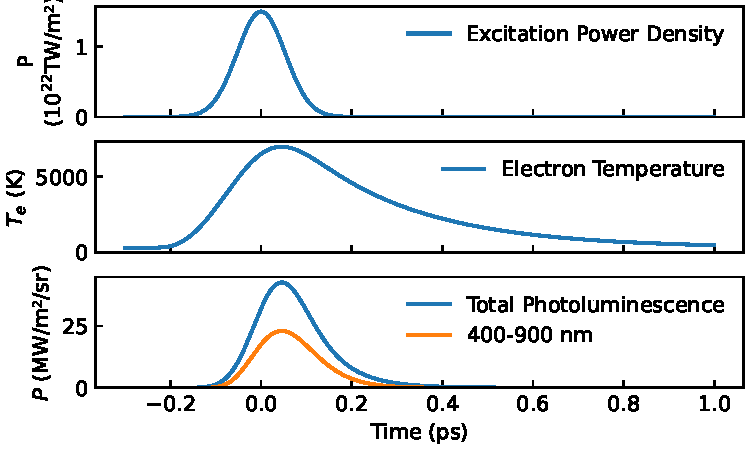
\includegraphics{../analysis/figures/model.time_evolution.pdf}
    \label{fig:timeevolution}
    \caption{}
\end{figure}
\begin{figure}[h]
    \centering
    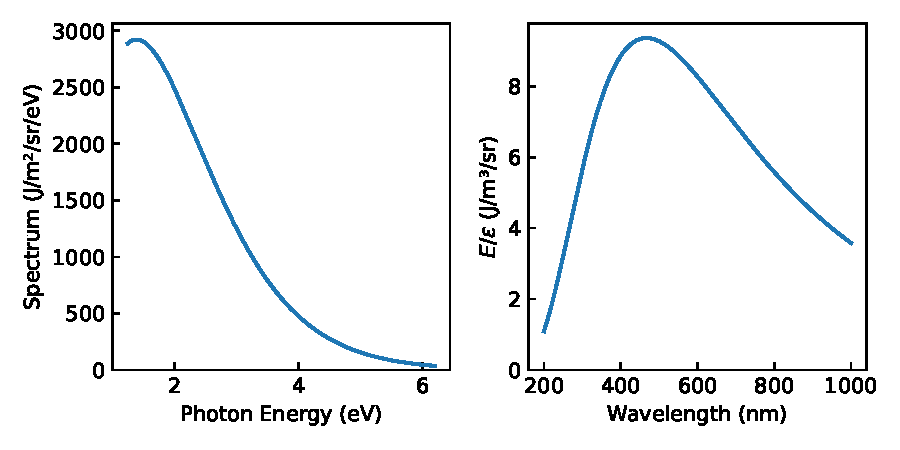
\includegraphics{../analysis/figures/model.spectrum.pdf}
    \label{fig:model_spectrum}
    \caption{}
\end{figure}
\begin{figure}[h]
    \centering
    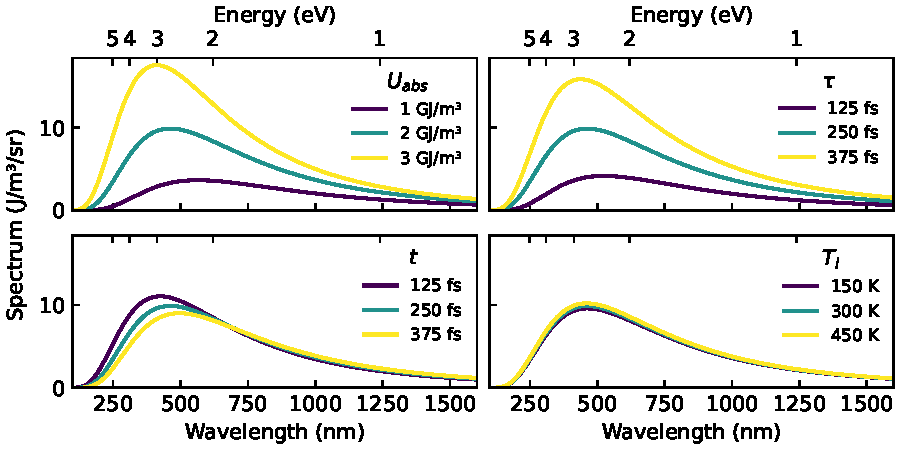
\includegraphics{../analysis/figures/sensitivity.pdf}
    \label{fig:sensitivity}
    \caption{}
\end{figure}
\begin{figure}[h]
    \centering
    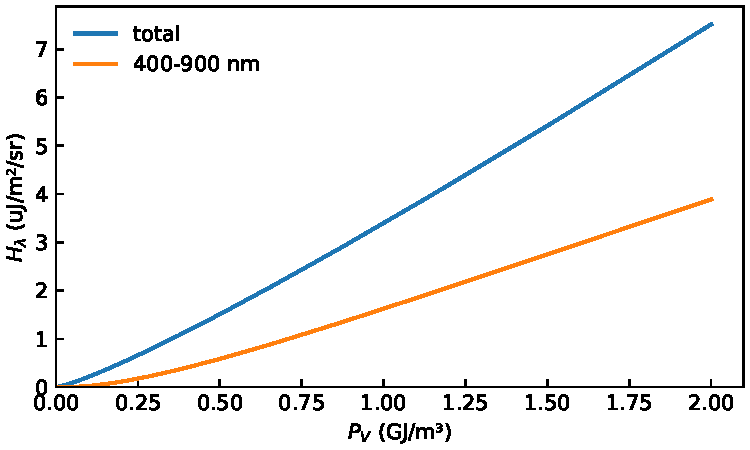
\includegraphics{../analysis/figures/powerscaling.pdf}
    \label{fig:powerscaling}
    \caption{}
\end{figure}


\clearpage
\section{Experimental Setup}
\begin{figure}[h]
    \centering
    \begin{subfigure}{3.5in}
        \centering
        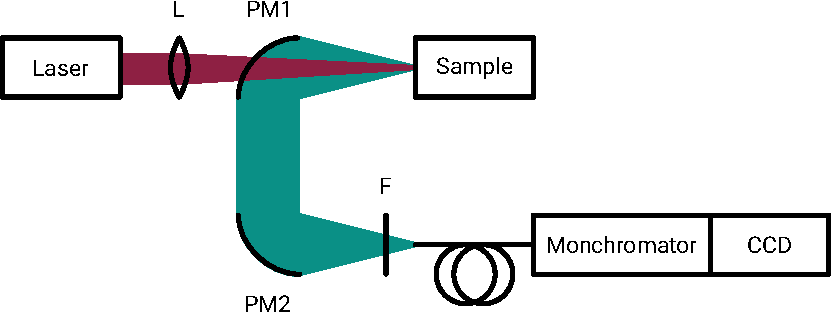
\includegraphics{figures/setup.pdf}
        \caption{Schematic}
    \end{subfigure}\hfill
    \begin{subfigure}{2in}
        \centering
        \includegraphics{figures/photo_setup.pdf}
        \caption{Photograph}
    \end{subfigure}
    \caption{Experimental setup used to measure thermal emission from ultrafast-excited hot electrons. The schematic shows the optical path and key components; the photograph shows the arrangement inside the chamber.}
    \label{fig:setup}
\end{figure}

The experimental setup, originally developed by Leon Roob~\cite{roobThermalRadiationUltrafast2025}, is shown in \autoref{fig:setup}. It is designed to measure broadband thermal emission from hot electrons in graphite using reflective collection optics and a fibre-coupled spectrometer.

The excitation source is a PHAROS PH1-20 (Light Conversion) at a centre wavelength of \SI{1030}{\nano\metre}, with pulse duration \SI{250}{\femto\second} (FWHM) and repetition rate \SI{40}{\kilo\hertz}. The pulse energy is \SI{7.5}{\micro\joule} (average power \SI{300}{\milli\watt}). The beam is stabilised in four axes and expanded to a diameter of $D=\SI{5}{\milli\metre}$ before entering the chamber.

Inside the chamber, a plano-convex lens with focal length \(f=\SI{200}{\milli\metre}\) focuses the beam onto the sample. Using the standard diffraction estimate \(d \approx 4\lambda f / \pi D\), the expected spot diameter is \(\gtrsim\SI{50}{\micro\metre}\).

The target is a graphite sample mounted on a three-axis translation stage. Thermal emission from the irradiated spot is collected by two off-axis parabolic mirrors (UV-enhanced aluminium). The first mirror (PM1, \(f=\SI{50}{\milli\metre}\)) collimates the emission; the second (PM2, \(f=\SI{101}{\milli\metre}\)) focuses it onto a band-pass filter and into a multimode fibre with a \SI{200}{\micro\metre} core (Ocean Optics QP200-2-SR-BX). The magnification is \(M = f_{\mathrm{PM2}}/f_{\mathrm{PM1}} \approx 2\), yielding an image spot of \(\sim\SI{100}{\micro\metre}\) at the fibre entrance, comfortably within the core.

The fibre feeds an Acton SpectraPro 300i monochromator equipped with a 150\,lines\,mm\(^{-1}\) grating blazed at \SI{500}{\nano\metre}. The dispersed spectrum is detected by an Andor iXon\textsuperscript{EM}+ 897 EMCCD operated in vertical binning mode, effectively serving as a 1D line detector.
Wavelength calibration (performed once following the manufacturer’s procedure~\cite{roobThermalRadiationUltrafast2025}) was stable throughout the measurements.

For alignment and maximal throughput, the lens, sample, and fibre ferrule are mounted on independent precision translation stages, while PM1 and PM2 are fixed on the common optical axis. 

\subsection{Noise and detector considerations}
Detecting the weak thermal radiation from hot electrons requires careful optimisation of the signal-to-noise ratio (SNR). In this setup the dominant noise sources originate from the detector; laser power fluctuations and mechanical variations are treated as negligible. The EMCCD mechanisms are well documented by Andor~\cite{dr.jowaltersSensitivityNoiseCCD2023,andorEstablishingSensitivityScientifica} and standards \cite{europeanmachinevisionassociationStandardCharacterizationImage2010}.

\textbf{Readout noise.}
This is the fundamental noise from charge transfer and A/D conversion. For the present camera, the fit in \autoref{fig:dark_noise} yields a constant read noise of
\(\sigma_{\text{read}}=\SI{0.81(12)}{DN}\), consistent with the manufacturer’s specification~\cite{andorIXonEM897Manual}.
Because read noise is applied per read out bin, hardware binning (1D line-detector mode) reduces its impact by summing signal prior to the single read.

\textbf{Dark current noise.}
Thermally generated charge scales with temperature and time,
\(N_\text{dark}\propto \exp(-E/kT)\,t_\text{exp}\).
\autoref{fig:dark_noise} shows the measured dependence; fitting gives an effective activation energy \(E=\SI{0.597(4)}{eV}\).
With the sensor cooled to \SI{-80}{\degreeCelsius}, the dark contribution is negligible at the exposure times used.

\begin{figure}[h]
    \centering
    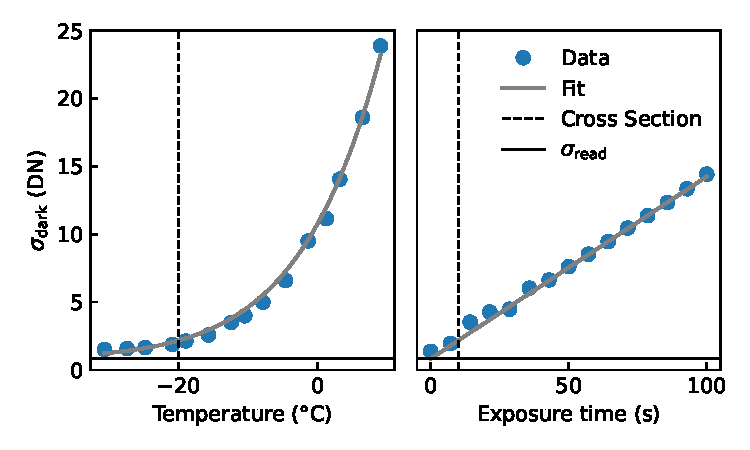
\includegraphics{../analysis/figures/dark_noise.pdf}
    \caption{Dark noise vs.\ sensor temperature and exposure time. Fit yields \(E=\SI{0.597(4)}{eV}\) and \(\sigma_{\text{read}}=\SI{0.81(12)}{e^{-}}\).}
    \label{fig:dark_noise}
\end{figure}

\textbf{Clock-induced charge (CIC).}
CIC is created during high-speed clocking.
Its apparent contribution grows with electron multiplication gain, so \emph{EM gain is disabled} in this work (signal levels are well above the read-noise floor), which keeps CIC negligible~\cite{andorEstablishingSensitivityScientifica}.

\textbf{Shot noise and photon-transfer method.}
Under these optimised conditions the dominant term is shot noise.
Incident photons create photoelectrons with quantum efficiency \(\eta\), so \(N_e=\eta\,N_{\text{photons}}\) and, for Poisson statistics, \(\operatorname{var}(N_e)=N_e\)~\cite{europeanmachinevisionassociationStandardCharacterizationImage2010}.
Let \(G\) denote the system conversion gain (DN per electron). The measured signal in data numbers (DN) is \(S = G\,N_e\), and the measured variance becomes \(\sigma^2_{\text{meas}} \;=\; \sigma_{\text{read}}^2 \;+\; G\,S\).
Thus a plot of variance vs.\ mean (photon-transfer curve) is linear in the shot-noise regime with slope \(G\).
\autoref{fig:shotnoise} shows this behaviour; from the slope \(G \approx 10~\text{DN}/e^{-}\) can be measured.
Note that this procedure does \emph{not} determine \(\eta\); it only gives the DN-to-electron conversion.

\begin{figure}[h]
    \centering
    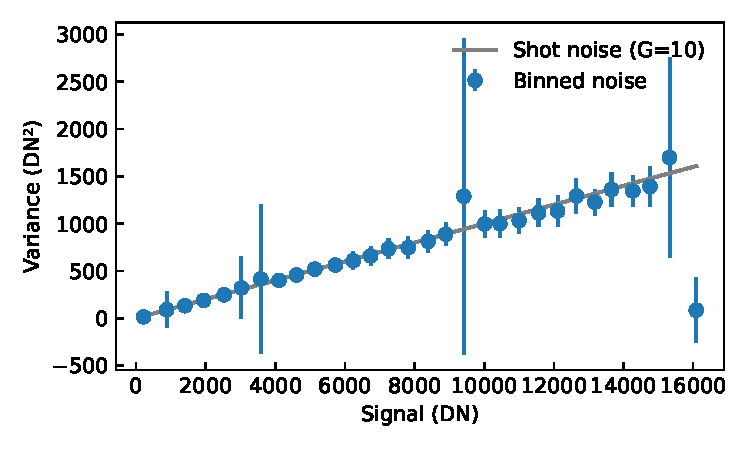
\includegraphics{../analysis/figures/shot noise.pdf}
    \caption{Measured noise vs.\ signal (photon-transfer curve) demonstrating shot-noise-limited operation; the linear slope yields the conversion gain \(G\).}
    \label{fig:shotnoise}
\end{figure}

\textbf{Practical settings for reproducibility.}
(1) Keep the camera at \(\leq\)\SI{-80}{\degreeCelsius}; (2) use vertical binning to treat the EMCCD as a 1D detector; (3) disable EM gain to avoid CIC and excess-noise-factor penalties; (4) fix slit width and exposure during noise characterisation; (5) verify the shot-noise regime by measuring \(\sigma^2\) vs.\ \(S\) and confirming linearity and slope \(G\)

\subsection{Focusing and Alignment}
The aim is to image the excited spot on the sample onto the spectrometer fibre with maximal throughput. Parabolic mirrors (PM1/PM2) remain fixed once set; all focusing is done with the lamp, fibre/spectrometer port, and sample stages.

\begin{enumerate}
  \item \textbf{Initial setup with a fiber coupled lamp.}  
  Remove the sample and place a fiber-coupled lamp at the sample position. This will help align and focus the optics using visible light.

  \item \textbf{Align the beam.}  
  Adjust the lamp position and the parabolic mirrors so that the beam appears circular and sharply focused at the spectrometer fiber port. This ensures the optics are approximately aligned.

  \item \textbf{Connect and optimize with spectrometer.}  
  Connect the spectrometer to the spectrometer port and move the holder to maximize the signal roughly. Use the micrometer screws on the sample stage for fine adjustments.

  \item \textbf{Swap back in the sample.}  
  Replace the lamp with the sample at the same position. Connect the lamp output to the spectrometer port to illuminate the sample.

  \item \textbf{Fine-focus the sample.}  
  Adjust the sample position to minimize the size of the visible spot on the sample.

  \item \textbf{Focus the infrared laser.}  
  Turn on the infrared laser and use an IR detection card to locate and focus the beam onto the sample. The white light and the IR be collinear.

  \item \textbf{Optimize laser alignment.}  
  Replace the lamp with the spectrometer and monitor the reflected laser signal on the spectrometer. Fine-tune the laser focus to maximize this signal.
\end{enumerate}

\subsection{Data processing}
All raw spectra were first corrected by subtracting a dark frame recorded with identical acquisition settings, removing the fixed electronic bias and dark current.  
Residual peaks at the fundamental and harmonic wavelengths of the pump laser, normally suppressed by laser line filters, were present due to the absence of suitable optical filtering.  
These peaks were identified and removed digitally, leaving gaps in the plotted spectra where the affected bins were excluded.  

The corrected signal \(S(\lambda)\) in DN was converted to spectral power density \(P_{\text{meas}}(\lambda)\) via
\begin{equation}
  P_{\text{meas}}(\lambda)
  = \frac{S(\lambda)}{G\,t_{\text{exp}}\,\Delta\lambda}\,\frac{hc}{\lambda},
\end{equation}
with \(G\) the DN/\(e^-\) conversion gain, \(t_{\text{exp}}\) the exposure time, and \(\Delta\lambda\) the spectral bin width.  

\clearpage
\section{Measurement}
\begin{figure}[h]
    \centering
    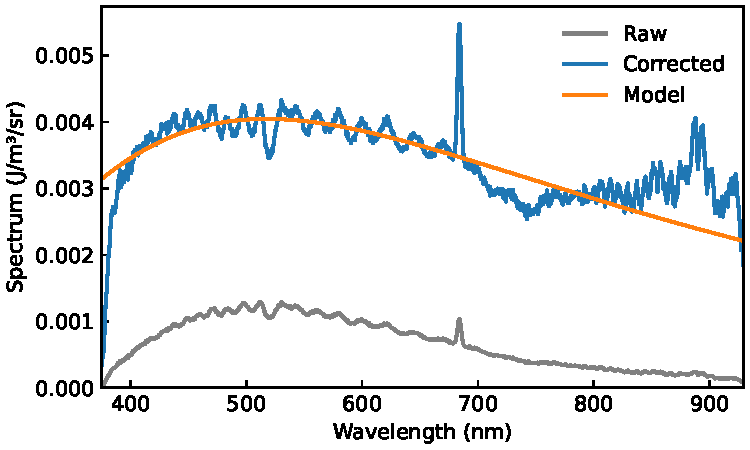
\includegraphics{../analysis/figures/combined.fit.pdf}
    \label{fig:fit}
    \caption{}
\end{figure}

\clearpage
\printbibliography

\end{document}